\section{Scalable Frequent-itemset Mining Methods}

\begin{frame}{The Downward-closure Property}

	\begin{block}{The Downward-closure Property}
		Any subset of a frequent itemset must also be frequent.
	\end{block}

	\begin{itemize}
		\item \textbf{Example:}

		      \begin{itemize}
			      \item If $\{\text{Beer, Diapers, Nuts}\}$ is frequent, so is $\{\text{Beer, Diapers}\}$.
			      \item I.e. every transaction having $\{\text{Beer, Diapers, Nuts}\}$ also contains $\{\text{Beer, Diapers}\}$.
		      \end{itemize}
		\item \textbf{Utilized by the major frequent-itemset mining algorithms:}
		      \begin{itemize}
			      \item Apriori\footnote{\fullcite{agarwal1994}}
			      \item Frequent-pattern growth (FP-growth)\footnote{\fullcite{han2000}}
			      \item etc \ldots
		      \end{itemize}
	\end{itemize}
\end{frame}

\subsection{Apriori}

\begin{frame}{Apriori Algorithm}
	\begin{block}{The Apriori Pruning Principle\footnote{\fullcite{agarwal1994}}\footnote{\fullcite{mannila1994}}}
		If there is any itemset which is infrequent, its supersets should not be generated/tested!
	\end{block}

	\begin{itemize}
		\item \textbf{The Apriori Algorithm - A Candidate Generation Approach:\footnote{A complete pseudo-code can be found in the appendix.}}
		      \begin{itemize}
			      \item Initially, scan DB once to get frequent $1$-itemsets.
			      \item Generate length-$(k+1)$ candidate itemsets from length-$k$
			            frequent itemsets.
			      \item Test the candidates against DB, discard those that are
			            infrequent.
			      \item Terminate when no further candidate or frequent itemset can
			            be generated.
		      \end{itemize}
	\end{itemize}
\end{frame}

\begin{frame}{Apriori Algorithm - Example}
	\centering
	\vspace{0cm}
	\scalebox{0.9}{%
		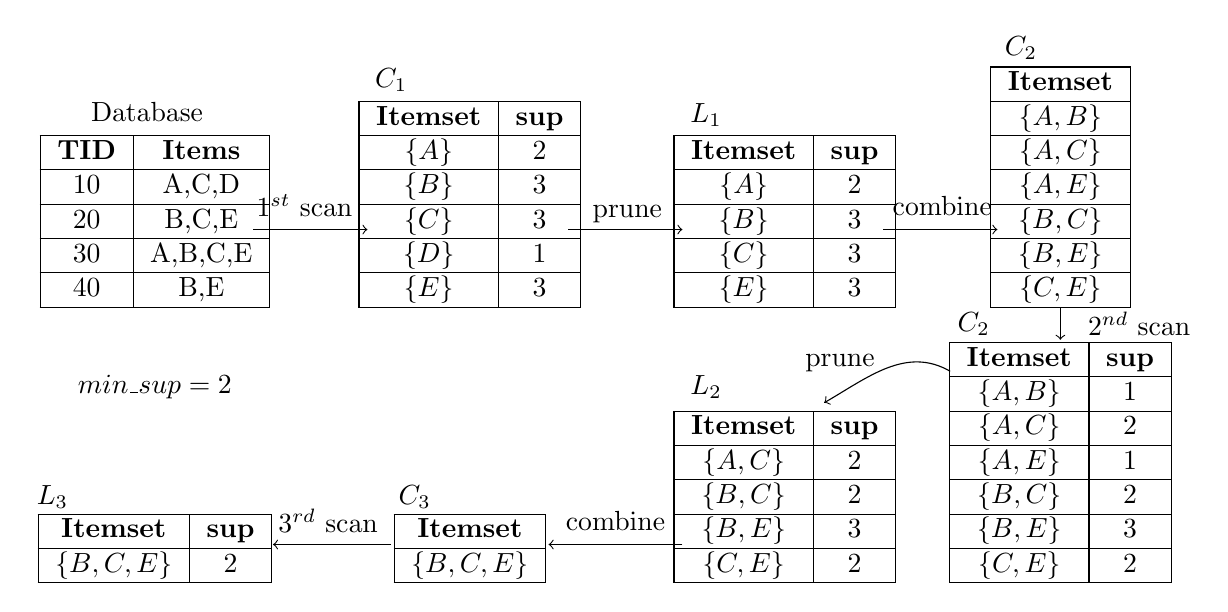
\begin{tikzpicture}
			\visible<1->{
				\path (0,1) coordinate (A) node[above, inner sep=0] {
						\begin{tabular}{ | c | c |}
							\hline
							\textbf{TID} & \textbf{Items} \\\hline
							10           & A,C,D          \\\hline
							20           & B,C,E          \\\hline
							30           & A,B,C,E        \\\hline
							40           & B,E            \\\hline
						\end{tabular}
					};
			}

			\visible<2->{
				\path (4,1) coordinate (A) node[above, inner sep=0] {
						\begin{tabular}{ | c | c |}
							\hline
							\textbf{Itemset} & \textbf{sup} \\\hline
							$\{A\}$          & 2            \\\hline
							$\{B\}$          & 3            \\\hline
							$\{C\}$          & 3            \\\hline
							$\{D\}$          & 1            \\\hline
							$\{E\}$          & 3            \\\hline
						\end{tabular}
					};
			}

			\visible<3->{
				\path (8,1) coordinate (A) node[above, inner sep=0] {
						\begin{tabular}{ | c | c |}
							\hline
							\textbf{Itemset} & \textbf{sup} \\\hline
							$\{A\}$          & 2            \\\hline
							$\{B\}$          & 3            \\\hline
							$\{C\}$          & 3            \\\hline
							$\{E\}$          & 3            \\\hline
						\end{tabular}
					};
			}

			\visible<4->{
				\path (11.5,1) coordinate (A) node[above, inner sep=0] {
						\begin{tabular}{ | c |}
							\hline
							\textbf{Itemset} \\\hline
							$\{A,B\}$        \\\hline
							$\{A,C\}$        \\\hline
							$\{A,E\}$        \\\hline
							$\{B,C\}$        \\\hline
							$\{B,E\}$        \\\hline
							$\{C,E\}$        \\\hline
						\end{tabular}
					};
			}

			\visible<5->{
				\path (11.5,-2.5) coordinate (A) node[above, inner sep=0] {
						\begin{tabular}{ | c | c |}
							\hline
							\textbf{Itemset} & \textbf{sup} \\\hline
							$\{A,B\}$        & 1            \\\hline
							$\{A,C\}$        & 2            \\\hline
							$\{A,E\}$        & 1            \\\hline
							$\{B,C\}$        & 2            \\\hline
							$\{B,E\}$        & 3            \\\hline
							$\{C,E\}$        & 2            \\\hline
						\end{tabular}
					};
			}

			\visible<6->{
				\path (8,-2.5) coordinate (A) node[above, inner sep=0] {
						\begin{tabular}{ | c | c |}
							\hline
							\textbf{Itemset} & \textbf{sup} \\\hline
							$\{A,C\}$        & 2            \\\hline
							$\{B,C\}$        & 2            \\\hline
							$\{B,E\}$        & 3            \\\hline
							$\{C,E\}$        & 2            \\\hline
						\end{tabular}
					};
			}

			\visible<7->{
				\path (4,-2.5) coordinate (A) node[above, inner sep=0] {
						\begin{tabular}{ | c |}
							\hline
							\textbf{Itemset} \\\hline
							$\{B,C,E\}$      \\\hline
						\end{tabular}
					};
			}

			\visible<8->{
				\path (0,-2.5) coordinate (A) node[above, inner sep=0] {
						\begin{tabular}{ | c | c |}
							\hline
							\textbf{Itemset} & \textbf{sup} \\\hline
							$\{B,C,E\}$      & 2            \\\hline
						\end{tabular}
					};
			}


			\visible<2->{
				\draw[->] (1.25,2) -- (2.7,2);
			}

			\visible<3->{
				\draw[->] (5.25,2) -- (6.7,2);
			}

			\visible<4->{
				\draw[->] (9.25,2) -- (10.7,2);
			}

			\visible<5->{
				\draw[->] (11.5,1) -- (11.5,0.6);
			}

			\visible<6->{
				\draw[->] (10.1,0.2) to [out=150,in=30] (8.5,-0.2);
			}

			\visible<7->{
				\draw[->] (6.7,-2) -- (5,-2);
			}

			\visible<8->{
				\draw[->] (3,-2) -- (1.5,-2);
			}


			\visible<1->{
				\node at (-0.1,3.5) {Database};
				\node at (0,0) {$min\_sup = 2$};
			}

			\visible<2->{
				\node at (1.9,2.3) {$1^{\text{st}}$ scan};
				\node at (3,3.9) {$C_1$};
			}

			\visible<3->{
				\node at (6,2.2) {prune};
				\node at (7,3.45) {$L_1$};
			}

			\visible<4->{
				\node at (10,2.3) {combine};
				\node at (11,4.3) {$C_2$};
			}

			\visible<5->{
				\node at (12.5,0.8) {$2^{\text{nd}}$ scan};
				\node at (10.4,0.8) {$C_2$};
			}

			\visible<6->{
				\node at (8.7,0.3) {prune};
				\node at (7,0) {$L_2$};
			}

			\visible<7->{
				\node at (3.3,-1.4) {$C_3$};
				\node at (5.85,-1.7) {combine};
			}

			\visible<8->{
				\node at (2.2,-1.7) {$3^{\text{rd}}$ scan};
				\node at (-1.3,-1.4) {$L_3$};
			}
		\end{tikzpicture}
	}
\end{frame}


\begin{frame}{Apriori Algorithm - Candidate Generation}
	\begin{alertblock}{Follow the Apriori Pruning Principle!}
		If \textbf{any} subset of an itemset you wish to generate is infrequent, it is \textbf{not} a valid candidate!
	\end{alertblock}

	\vspace{0.25cm}

	\begin{itemize}
		\item \textbf{Example}\footnote{Based on the previous slide/example}\textbf{:}
		      \begin{itemize}
			      \item The itemset $\{A,B,C\}$ is \textbf{not} a valid candidate:
			            \begin{itemize}
				            \item Frequent Subsets: $\{A\}$, $\{B\}$, $\{C\}$, $\{A,C\}$, $\{B,C\}$
				            \item Infrequent Subset: $\{A,B\}$
			            \end{itemize}
		      \end{itemize}
		\item \textbf{\color{airforceblue}How to generate candidates?}
		      \begin{itemize}
			      \item Step 1: Join all frequent $k$-itemsets that have $k-1$ items in
			            common.
			            \begin{itemize}
				            \item E.g. $\{A,B\}$ and $\{A,C\}$ can be joined to form $\{A,B,C\}$.
			            \end{itemize}
			      \item Step 2: Prune all combinations that have infrequent subsets.
			            \begin{itemize}
				            \item E.g. $\{A,B,C\}$ has to be pruned, because $\{A,B\}$ is infrequent.
			            \end{itemize}
		      \end{itemize}
	\end{itemize}
\end{frame}

\begin{frame}{Improvements}
	\begin{itemize}
		\item \textbf{Apriori is pretty inefficient:}
		      \begin{itemize}
			      \item Multiple scans of transaction database.
			      \item Huge number of candidates.
			      \item Support counting for candidates is laborious.
		      \end{itemize}
		\item \textbf{Many improvements have been proposed.}
		\item \textbf{Some examples:}
		      \begin{itemize}
			      \item Reducing the passes of database scans:
			            \begin{itemize}
				            \item Partitioning\footnote{e.g. \fullcite{savasere1995}}
				            \item Dynamic itemset counting\footnote{e.g. \fullcite{brin1997}}
			            \end{itemize}
			      \item Shrinking the number of candidates:
			            \begin{itemize}
				            \item Hashing\footnote{e.g. \fullcite{park1995}}
			            \end{itemize}
		      \end{itemize}
	\end{itemize}
\end{frame}

\begin{frame}{Improvements - Partitioning}
	\begin{block}{Partitioning: The Basic Idea}
		Any itemset that is potentially frequent in the whole database must be frequent in at least one of the partitions of the database.
	\end{block}
	\begin{itemize}
		\item \textbf{Method: Scan the database twice}
		      \begin{itemize}
			      \item Scan 1: Partition database and find the local frequent itemsets:
			            \begin{itemize}
				            \item $\text{min\_sup}_i = \text{min\_sup}[\%] \cdot \vert
					                  \sigma\text{DB}_i \vert$.
			            \end{itemize}
			      \item Scan 2: Use the local frequent itemsets to check for global frequent itemsets:
			            \begin{itemize}
				            \item Only itemsets that are frequent in at least one partition are checked.
			            \end{itemize}
		      \end{itemize}
	\end{itemize}
	\vspace{0.25cm}
	\centering
	\begin{tikzpicture}[square/.style={regular polygon,regular polygon sides=4}]
		\node at (0,0) [square, draw, fill=gray, minimum size=2cm] {};
		\node at (3,0) [square, draw, fill=gray, minimum size=2cm] {};
		\node at (8,0) [square, draw, fill=gray, minimum size=2cm] {};
		\node at (5.5,0) {$\hdots$};
		\node at (0,0) {DB$_1$};
		\node at (0,-1.5) {$\sup_1(i) \leq \vert\sigma \text{DB}_1\vert$};
		\node at (3,-1.5) {$\sup_2(i) \leq \vert\sigma \text{DB}_2\vert$};
		\node at (8,-1.5) {$\sup_k(i) \leq \vert\sigma \text{DB}_k\vert$};
		\node at (10.5,-0.5) {$\sup(i) \leq \vert\sigma \text{DB}\vert$};
		\node at (3,0) {DB$_2$};
		\node at (8,0) {DB$_k$};
		\node at (4.5,0) {+};
		\node at (6.5,0) {+};
		\node at (1.5,0) {+};
		\node at (10,0) {= DB};
	\end{tikzpicture}
\end{frame}

\begin{frame}{Improvements - Dynamic Itemset Counting (I)}
	\begin{block}{Dynamic Itemset Counting (DIC): The Basic Idea}
		Itemset frequency counting starts once all subsets are confirmed to be frequent.
	\end{block}

	\begin{itemize}
		\item \textbf{Candidate itemsets are added at different points during a scan:}
		      \begin{itemize}
			      \item New candidate itemsets can be added at any start point during a scan.
			            \begin{itemize}
				            \item E.g. if $A$ and $B$ are already found to be frequent, \\
				                  $AB$ are also counted from that starting point on.
			            \end{itemize}
			      \item Uses the count-so-far as the lower bound of the actual count.
			      \item If count-so-far passes minimum support, itemset is added to
			            frequent-itemset collection.
			      \item Can then be used to generate even longer candidates.
		      \end{itemize}
	\end{itemize}
\end{frame}

\begin{frame}{Improvements - Dynamic Itemset Counting (II)}
	\vspace{1cm}
	\begin{columns}
		\begin{column}{0.5\textwidth}
			\centering
			\scalebox{0.9}{
				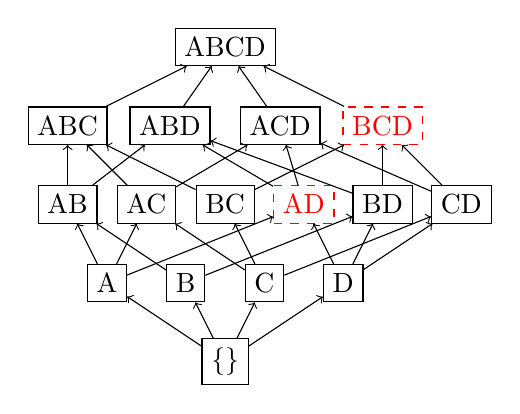
\begin{tikzpicture}
					\node[draw] at (0,0) (abcd) {ABCD};
					\node[draw] at (-2,-1) (abc) {ABC};
					\node[draw] at (-0.7,-1) (abd) {ABD};
					\node[draw] at (0.7,-1) (acd) {ACD};
					\node[draw, dashed, color=red] at (2,-1) (bcd) {BCD};

					\node[draw] at (-2,-2) (ab) {AB};
					\node[draw] at (-1,-2) (ac) {AC};
					\node[draw] at (0,-2) (bc) {BC};
					\node[draw, dashed, color=red] at (1,-2) (ad) {AD};
					\node[draw] at (2,-2) (bd) {BD};
					\node[draw] at (3,-2) (cd) {CD};

					\node[draw] at (-1.5,-3) (a) {A};
					\node[draw] at (-0.5,-3) (b) {B};
					\node[draw] at (0.5,-3) (c) {C};
					\node[draw] at (1.5,-3) (d) {D};
					\node[draw] at (0,-4) (0) {$\{\}$};

					\draw[->] (0)-- (a);
					\draw[->] (0)-- (b);
					\draw[->] (0)-- (c);
					\draw[->] (0)-- (d);
					\draw[->] (a)-- (ab);
					\draw[->] (a)-- (ac);
					\draw[->] (a)-- (ad);
					\draw[->] (b)-- (ab);
					\draw[->] (b)-- (bd);
					\draw[->] (c)-- (ac);
					\draw[->] (c)-- (bc);
					\draw[->] (c)-- (cd);
					\draw[->] (d)-- (ad);
					\draw[->] (d)-- (bd);
					\draw[->] (d)-- (cd);

					\draw[->] (ab)-- (abc);
					\draw[->] (ab)-- (abd);
					\draw[->] (ac)-- (abc);
					\draw[->] (ac)-- (acd);
					\draw[->] (bc)-- (abc);
					\draw[->] (bc)-- (bcd);
					\draw[->] (ad)-- (abd);
					\draw[->] (ad)-- (acd);
					\draw[->] (bd)-- (abd);
					\draw[->] (bd)-- (bcd);
					\draw[->] (cd)-- (acd);
					\draw[->] (cd)-- (bcd);

					\draw[->] (abc)-- (abcd);
					\draw[->] (abd)-- (abcd);
					\draw[->] (acd)-- (abcd);
					\draw[->] (bcd)-- (abcd);
				\end{tikzpicture}
			}
		\end{column}
		\begin{column}{0.5\textwidth}
			\vspace{-6.2cm}
			\scalebox{0.9}{
				\begin{tikzpicture}
					\node[draw, fill=gray, text width = 7cm]
					{\color{white}Transactions};
					\draw[->, color=airforceblue] (-3,-0.8) -- (3,-0.8);
					\draw[->, color=airforceblue] (-3,-1.3) -- (3,-1.3);
					\draw[->, color=airforceblue] (-3,-1.8) -- (3,-1.8);
					\draw[->, color=red] (-3,-2.3) -- (3,-2.3);
					\draw[color=red] (-2,-2.8) -- (3,-2.8);
					\draw[color=red] (0,-3.3) -- (3,-3.3);
					\draw[->, color=red] (-3,-3.8) -- (-1.5,-3.8);
					\draw[->, color=red] (-3,-4.3) -- (0.5,-4.3);
					\node at (0, -0.5) {\color{airforceblue}1-itemsets};
					\node at (0, -1.1) {\color{airforceblue}2-itemsets};
					\node at (0, -2.1) {\color{red}1-itemsets};
					\node at (0, -2.6) {\color{red}2-itemsets};
					\node at (0.8, -3.1) {\color{red}3-itemsets};
					\node at (0, -1.6) {\color{airforceblue}$\ldots$};
					\draw[dashed, color=red] (3,-2.8) -- (-3,-3.8);
					\draw[dashed, color=red] (3,-3.3) -- (-3,-4.3);
					\node at (-3.5, -3.1) {\color{red}DIC:};
					\node at (-3.5, -1.1) {\color{airforceblue}Apriori:};
				\end{tikzpicture}
			}
		\end{column}
	\end{columns}
\end{frame}

\begin{frame}{Improvements - Hashing}
	\begin{block}{Hashing: The Basic Idea}
		Itemsets are hashed into buckets, and during the first scan, only the occurrences of each bucket are counted.
	\end{block}

	\begin{columns}[c]
		\begin{column}{0.6\textwidth}
			\begin{itemize}
				\item \textbf{A $k$-itemset whose corresponding hashing-bucket
					      count is below the threshold cannot be frequent.}
				      \begin{itemize}
					      \item Candidates: $a,b,c,d,e$.
					      \item While scanning DB for frequent $1$-itemsets, create
					            hash entries for $2$-itemsets:
					            \begin{itemize}
						            \item $\{ab,ad,ae\}$
						            \item $\{bd,be,de\}$
						            \item $\ldots$
					            \end{itemize}
					      \item Frequent $1$-itemset: $a,b,d,e$.
					      \item $ab$ is not a candidate $2$-itemset, if the sum of
					            count of $\{ab, ad, ae\}$ is below support threshold.
				      \end{itemize}
			\end{itemize}
		\end{column}
		\begin{column}{0.3\textwidth}
			\centering
			\textbf{Hash table:}\\
			\begin{tabular}{| c | c |}
				\hline
				count    & itemsets       \\\hline
				35       & $\{ab,ad,ae\}$ \\\hline
				88       & $\{bd,be,de\}$ \\\hline
				$\vdots$ & $\vdots$       \\\hline
				102      & $\{yz,qs,wt\}$ \\\hline
			\end{tabular}
		\end{column}
	\end{columns}
\end{frame}

\subsection{FP-growth}

\begin{frame}{FP-growth}
	\begin{itemize}
		\item \textbf{Bottlenecks of the Apriori approach.}
		      \begin{itemize}
			      \item Breadth-first (i.e., level-wise) search.
			      \item Candidate generation and test.
			            \begin{itemize}
				            \item Often generates a huge number of candidates.
			            \end{itemize}
		      \end{itemize}
		\item \textbf{The FP-growth Approach.} (Han, Pei \& Yin, SIGMOD'00)
		      \begin{itemize}
			      \item Depth-first search.
			      \item Avoid explicit candidate generation.
		      \end{itemize}
		\item \textbf{Major philosophy: Grow long patterns from short ones
			      using local frequent items only.}
		      \begin{itemize}
			      \item $abc$ is a frequent pattern.
			      \item Get all transactions having $abc$, i.e. restrict DB on $abc$:
			            $DB|_{abc}$.
			      \item $d$ is a local frequent item in $DB|_{abc \implies abcd}$ is
			            a frequent pattern.
		      \end{itemize}
	\end{itemize}
\end{frame}

\begin{frame}{Construct FP-tree from a Transaction Database}
	\centering
	\begin{tabular}{|c|c|c|}
		\hline
		\underline{TID} & \underline{Items bought} & \underline{(ordered)
		frequent items}                                                   \\\hline
		100             & $\{f,a,c,d,g,i,m,p\}$    & $\{f,c,a,m,p\}$      \\\hline
		200             & $\{a,b,c,f,l,m\}$        & $\{f,c,a,b,m\}$      \\\hline
		300             & $\{b,f,h,j,o,w\}$        & $\{f,b\}$            \\\hline
		400             & $\{b,c,k,s,p\}$          & $\{c,b,p\}$          \\\hline
		500             & $\{a,f,c,e,l,p,m,n\}$    & $\{f,c,a,m,p\}$      \\\hline
	\end{tabular}
	\vspace{0.2cm}
	\begin{columns}
		\begin{column}{0.5\textwidth}
			\vspace{-3.5cm}
			\begin{itemize}
				\item[1.] Scan DB once, find frequent $1$-itemsets (single-item
				      patterns).
				\item[2.] Sort frequent items in frequency-descending order,
				      creating the \textbf{f-list}.
				\item[3.] Scan DB again, construct \textbf{FP-tree}.
			\end{itemize}
		\end{column}
		\begin{column}{0.5\textwidth}
			\centering
			\scalebox{0.85}{
				\begin{tikzpicture}
					\node[draw, fill=airforceblue] at (0,0) (0)
					{\color{white}$\{\}$};
					\node[draw, fill=airforceblue] at (-1,-0.7) (f4)
					{\color{white}$f:4$};
					\node[draw, fill=airforceblue] at (-1.5,-1.4) (c3)
					{\color{white}$c:3$};
					\node[draw, fill=airforceblue] at (-1.5,-2.1) (a3)
					{\color{white}$a:3$};
					\node[draw, fill=airforceblue] at (-2,-2.7) (m2)
					{\color{white}$m:2$};
					\node[draw, fill=airforceblue] at (-2,-3.3) (p2)
					{\color{white}$p:2$};
					\node[draw, fill=airforceblue] at (-1,-2.7) (b12)
					{\color{white}$b:1$};
					\node[draw, fill=airforceblue] at (-1,-3.3) (m1)
					{\color{white}$m:1$};

					\node[draw, fill=airforceblue] at (-0.5,-1.4) (b1)
					{\color{white}$b:1$};
					\node[draw, fill=airforceblue] at (1,-0.7) (c1)
					{\color{white}$c:1$};
					\node[draw, fill=airforceblue] at (1,-1.4) (b13)
					{\color{white}$b:1$};
					\node[draw, fill=airforceblue] at (1,-2.1) (p1)
					{\color{white}$p:1$};
					\draw (0) -- (f4) -- (c3) -- (a3) -- (m2) -- (p2);
					\draw (0) -- (c1);
					\draw (f4) -- (b1);
					\draw (a3) -- (b12) -- (m1);
					\draw (c1) -- (b13) -- (p1);
					\node at (2,0) (0)
					{\color{airforceblue}$\text{min\_sup}=3$};
					\node at (2,-3) (0) {\textbf{\color{airforceblue}F-list} =
						f-c-a-b-m-p};
				\end{tikzpicture}
			}
		\end{column}
	\end{columns}
\end{frame}

\begin{frame}{Partition Itemsets and Databases}
	\begin{itemize}
		\item \textbf{Frequent itemsets can be partitioned into subsets
			      according to f-list.}
		      \begin{itemize}
			      \item F-list = f-c-a-b-m-p.
			      \item Patterns containing p.
			            \begin{itemize}
				            \item The least-frequent item (at the end of the f-list,
				                  suffix).
			            \end{itemize}
			      \item Patterns having m but not p.
			      \item $\vdots$
			      \item Patterns having c but not a nor b, m, p.
			      \item Pattern f.
		      \end{itemize}
		\item \textbf{This processing order guarantees completeness and
			      non-redundancy.}
	\end{itemize}
\end{frame}

\begin{frame}{Find Itemsets from $p$'s Conditional Pattern Base}
	\begin{itemize}
		\item \textbf{Starting at the frequent-item header table in the
			      FP-tree.}
		\item \textbf{Traverse the FP-tree by following the link of frequent
			      item $p$.}
		\item \textbf{Accumulate all transformed {\color{airforceblue}prefix
				      paths} of item $p$ to form $p$'s {\color{red}conditional pattern base}.}
	\end{itemize}
	\vspace{0.2cm}
	\centering
	\scalebox{0.9}{
		\begin{tikzpicture}
			\node[draw, fill=airforceblue] at (0,0) (0) {\color{white}$\{\}$};
			\node[draw, fill=airforceblue] at (-1,-0.7) (f4)
			{\color{white}$f:4$};
			\node[draw, fill=airforceblue] at (-1.5,-1.4) (c3)
			{\color{white}$c:3$};
			\node[draw, fill=airforceblue] at (-1.5,-2.1) (a3)
			{\color{white}$a:3$};
			\node[draw, fill=airforceblue] at (-2,-2.7) (m2)
			{\color{white}$m:2$};
			\node[draw, fill=airforceblue] at (-2,-3.3) (p2)
			{\color{white}$p:2$};
			\node[draw, fill=airforceblue] at (-1,-2.7) (b12)
			{\color{white}$b:1$};
			\node[draw, fill=airforceblue] at (-1,-3.3) (m1)
			{\color{white}$m:1$};

			\node[draw, fill=airforceblue] at (-0.5,-1.4) (b1)
			{\color{white}$b:1$};
			\node[draw, fill=airforceblue] at (1,-0.7) (c1)
			{\color{white}$c:1$};
			\node[draw, fill=airforceblue] at (1,-1.4) (b13)
			{\color{white}$b:1$};
			\node[draw, fill=airforceblue] at (1,-2.1) (p1)
			{\color{white}$p:1$};
			\draw (0) -- (f4) -- (c3) -- (a3) -- (m2) -- (p2);
			\draw (0) -- (c1);
			\draw (f4) -- (b1);
			\draw (a3) -- (b12) -- (m1);
			\draw (c1) -- (b13) -- (p1);
			\node at (2,0) (0) {\color{airforceblue}$\text{min\_sup}=3$};
			\node at (2,-3) (0) {\textbf{\color{airforceblue}F-list} =
				f-c-a-b-m-p};
			\node at (5.5,0.5) (0) {\textbf{Header table:}};
			\node at (10,0.5) (0) {\textbf{Conditional pattern bases:}};
			\node at (5.5,-1.5) (0) {
				\begin{tabular}{|c|c|}
					\hline
					\textbf{item} & \textbf{Frequency} \\\hline
					f             & 4                  \\
					c             & 4                  \\
					a             & 3                  \\
					b             & 3                  \\
					m             & 3                  \\
					p             & 3                  \\\hline
				\end{tabular}
			};
			\node at (10,-1.5) (0) {
				\begin{tabular}{|c|c|}
					\hline
					\textbf{item} & \textbf{pattern base} \\\hline
					c             & f:3                   \\
					a             & fc:3                  \\
					b             & fca:1, f:1, c:1       \\
					m             & fca:2, fcab:1         \\
					p             & fcam:2, cb:1          \\
					\hline
				\end{tabular}
			};
		\end{tikzpicture}
	}
\end{frame}

\begin{frame}{$p$'s Conditional Pattern Base}
	\centering
	\begin{tikzpicture}
		\node[draw, fill=airforceblue] at (0,0) (0) {\color{white}$\{\}$};
		\node[draw, fill=ForestGreen] at (-1,-0.7) (f4) {\color{white}$f:4$};
		\node[draw, fill=ForestGreen] at (-1.5,-1.4) (c3) {\color{white}$c:3$};
		\node[draw, fill=ForestGreen] at (-1.5,-2.1) (a3) {\color{white}$a:3$};
		\node[draw, fill=ForestGreen] at (-2,-2.7) (m2) {\color{white}$m:2$};
		\node[draw, fill=red] at (-2,-3.3) (p2) {\color{white}$p:2$};
		\node[draw, fill=airforceblue] at (-1,-2.7) (b12) {\color{white}$b:1$};
		\node[draw, fill=airforceblue] at (-1,-3.3) (m1) {\color{white}$m:1$};

		\node[draw, fill=airforceblue] at (-0.5,-1.4) (b1) {\color{white}$b:1$};
		\node[draw, fill=ForestGreen] at (1,-0.7) (c1) {\color{white}$c:1$};
		\node[draw, fill=ForestGreen] at (1,-1.4) (b13) {\color{white}$b:1$};
		\node[draw, fill=red] at (1,-2.1) (p1) {\color{white}$p:1$};
		\draw (0) -- (f4) -- (c3) -- (a3) -- (m2) -- (p2);
		\draw (0) -- (c1);
		\draw (f4) -- (b1);
		\draw (a3) -- (b12) -- (m1);
		\draw (c1) -- (b13) -- (p1);
		\node at (5.5,0.5) (0) {\textbf{Header table:}};
		\node at (5.5,-1.5) (0) {
			\begin{tabular}{|c|c|}
				\hline
				\textbf{item}         & \textbf{Frequency}    \\\hline
				f                     & 4                     \\
				c                     & 4                     \\
				a                     & 3                     \\
				b                     & 3                     \\
				m                     & 3                     \\
				\textbf{\color{red}p} & \textbf{\color{red}3} \\\hline
			\end{tabular}
		};
	\end{tikzpicture}\\[0.2cm]
	Hence, $p$'s conditional pattern base is\\
	fcam:2, cb:1\\
	both below min\_sup.
\end{frame}

\begin{frame}{$m$'s Conditional Pattern Base}
	\centering
	\begin{tikzpicture}
		\node[draw, fill=airforceblue] at (0,0) (0) {\color{white}$\{\}$};
		\node[draw, fill=ForestGreen] at (-1,-0.7) (f4) {\color{white}$f:4$};
		\node[draw, fill=ForestGreen] at (-1.5,-1.4) (c3) {\color{white}$c:3$};
		\node[draw, fill=ForestGreen] at (-1.5,-2.1) (a3) {\color{white}$a:3$};
		\node[draw, fill=red] at (-2,-2.7) (m2) {\color{white}$m:2$};
		\node[draw, fill=airforceblue] at (-2,-3.3) (p2) {\color{white}$p:2$};
		\node[draw, fill=ForestGreen] at (-1,-2.7) (b12) {\color{white}$b:1$};
		\node[draw, fill=red] at (-1,-3.3) (m1) {\color{white}$m:1$};

		\node[draw, fill=airforceblue] at (-0.5,-1.4) (b1) {\color{white}$b:1$};
		\node[draw, fill=airforceblue] at (1,-0.7) (c1) {\color{white}$c:1$};
		\node[draw, fill=airforceblue] at (1,-1.4) (b13) {\color{white}$b:1$};
		\node[draw, fill=airforceblue] at (1,-2.1) (p1) {\color{white}$p:1$};
		\draw (0) -- (f4) -- (c3) -- (a3) -- (m2) -- (p2);
		\draw (0) -- (c1);
		\draw (f4) -- (b1);
		\draw (a3) -- (b12) -- (m1);
		\draw (c1) -- (b13) -- (p1);
		\node at (5.5,0.5) (0) {\textbf{Header table:}};
		\node at (5.5,-1.5) (0) {
			\begin{tabular}{|c|c|}
				\hline
				\textbf{item}         & \textbf{Frequency}    \\\hline
				f                     & 4                     \\
				c                     & 4                     \\
				a                     & 3                     \\
				b                     & 3                     \\
				\textbf{\color{red}m} & \textbf{\color{red}3} \\
				p                     & 3                     \\\hline
			\end{tabular}
		};
	\end{tikzpicture}\\[0.2cm]
	Hence, $m$'s conditional pattern base is\\
	fca:2, fcab:1\\
	both below min\_sup.
\end{frame}

\begin{frame}{$b$'s Conditional Pattern Base}
	\centering
	\begin{tikzpicture}
		\node[draw, fill=airforceblue] at (0,0) (0) {\color{white}$\{\}$};
		\node[draw, fill=ForestGreen] at (-1,-0.7) (f4) {\color{white}$f:4$};
		\node[draw, fill=ForestGreen] at (-1.5,-1.4) (c3) {\color{white}$c:3$};
		\node[draw, fill=ForestGreen] at (-1.5,-2.1) (a3) {\color{white}$a:3$};
		\node[draw, fill=airforceblue] at (-2,-2.7) (m2) {\color{white}$m:2$};
		\node[draw, fill=airforceblue] at (-2,-3.3) (p2) {\color{white}$p:2$};
		\node[draw, fill=red] at (-1,-2.7) (b12) {\color{white}$b:1$};
		\node[draw, fill=airforceblue] at (-1,-3.3) (m1) {\color{white}$m:1$};

		\node[draw, fill=red] at (-0.5,-1.4) (b1) {\color{white}$b:1$};
		\node[draw, fill=ForestGreen] at (1,-0.7) (c1) {\color{white}$c:1$};
		\node[draw, fill=red] at (1,-1.4) (b13) {\color{white}$b:1$};
		\node[draw, fill=airforceblue] at (1,-2.1) (p1) {\color{white}$p:1$};
		\draw (0) -- (f4) -- (c3) -- (a3) -- (m2) -- (p2);
		\draw (0) -- (c1);
		\draw (f4) -- (b1);
		\draw (a3) -- (b12) -- (m1);
		\draw (c1) -- (b13) -- (p1);
		\node at (5.5,0.5) (0) {\textbf{Header table:}};
		\node at (5.5,-1.5) (0) {
			\begin{tabular}{|c|c|}
				\hline
				\textbf{item}         & \textbf{Frequency}    \\\hline
				f                     & 4                     \\
				c                     & 4                     \\
				a                     & 3                     \\
				\textbf{\color{red}b} & \textbf{\color{red}3} \\
				m                     & 3                     \\
				p                     & 3                     \\\hline
			\end{tabular}
		};
	\end{tikzpicture}\\[0.2cm]
	Hence, $b$'s conditional pattern base is\\
	fca:1, f:1, c:1\\
	{all below min\_sup.}
\end{frame}

\begin{frame}{$a$'s Conditional Pattern Base}
	\centering
	\begin{tikzpicture}
		\node[draw, fill=airforceblue] at (0,0) (0) {\color{white}$\{\}$};
		\node[draw, fill=ForestGreen] at (-1,-0.7) (f4) {\color{white}$f:4$};
		\node[draw, fill=ForestGreen] at (-1.5,-1.4) (c3) {\color{white}$c:3$};
		\node[draw, fill=red] at (-1.5,-2.1) (a2) {\color{white}$a:3$};
		\node[draw, fill=airforceblue] at (-2,-2.7) (m3) {\color{white}$m:3$};
		\node[draw, fill=airforceblue] at (-2,-3.3) (p2) {\color{white}$p:2$};
		\node[draw, fill=airforceblue] at (-1,-2.7) (b12) {\color{white}$b:1$};
		\node[draw, fill=airforceblue] at (-1,-3.3) (m1) {\color{white}$m:1$};

		\node[draw, fill=airforceblue] at (-0.5,-1.4) (b1) {\color{white}$b:1$};
		\node[draw, fill=airforceblue] at (1,-0.7) (c1) {\color{white}$c:1$};
		\node[draw, fill=airforceblue] at (1,-1.4) (b13) {\color{white}$b:1$};
		\node[draw, fill=airforceblue] at (1,-2.1) (p1) {\color{white}$p:1$};
		\draw (0) -- (f4) -- (c3) -- (a3) -- (m2) -- (p2);
		\draw (0) -- (c1);
		\draw (f4) -- (b1);
		\draw (a3) -- (b12) -- (m1);
		\draw (c1) -- (b13) -- (p1);
		\node at (5.5,0.5) (0) {\textbf{Header table:}};
		\node at (5.5,-1.5) (0) {
			\begin{tabular}{|c|c|}
				\hline
				\textbf{item}         & \textbf{Frequency}    \\\hline
				f                     & 4                     \\
				c                     & 4                     \\
				\textbf{\color{red}a} & \textbf{\color{red}3} \\
				b                     & 3                     \\
				m                     & 3                     \\
				p                     & 3                     \\\hline
			\end{tabular}
		};
	\end{tikzpicture}\\[0.2cm]
	Hence, $a$'s conditional pattern base is\\
	fc:3\\
	{has min\_sup.}
\end{frame}

\begin{frame}{From Conditional Pattern Bases to Conditional FP-trees}
	\centering
	\begin{itemize}
		\item \textbf{For each conditional pattern base:}
		      \begin{itemize}
			      \item Accumulate the count for each item in the base.
			      \item Construct the conditional FP-tree for the frequent items of
			            the pattern base.
		      \end{itemize}
	\end{itemize}
	\centering
	\scalebox{0.9}{
		\begin{tikzpicture}
			\node[draw, fill=airforceblue] at (0,0) (0) {\color{white}$\{\}$};
			\node[draw, fill=airforceblue] at (-1,-0.7) (f4)
			{\color{white}$f:4$};
			\node[draw, fill=airforceblue] at (-1.5,-1.4) (c2)
			{\color{white}$c:3$};
			\node[draw, fill=airforceblue] at (-1.5,-2.1) (a2)
			{\color{white}$a:3$};
			\node[draw, fill=airforceblue] at (-2,-2.7) (m2)
			{\color{white}$m:2$};
			\node[draw, fill=airforceblue] at (-2,-3.3) (p2)
			{\color{white}$p:2$};
			\node[draw, fill=airforceblue] at (-1,-2.7) (b12)
			{\color{white}$b:1$};
			\node[draw, fill=airforceblue] at (-1,-3.3) (m1)
			{\color{white}$m:1$};

			\node[draw, fill=airforceblue] at (-0.5,-1.4) (b1)
			{\color{white}$b:1$};
			\node[draw, fill=airforceblue] at (1,-0.7) (c1)
			{\color{white}$c:1$};
			\node[draw, fill=airforceblue] at (1,-1.4) (b13)
			{\color{white}$b:1$};
			\node[draw, fill=airforceblue] at (1,-2.1) (p1)
			{\color{white}$p:1$};
			\draw (0) -- (f4) -- (c3) -- (a3) -- (m2) -- (p2);
			\draw (0) -- (c1);
			\draw (f4) -- (b1);
			\draw (a3) -- (b12) -- (m1);
			\draw (c1) -- (b13) -- (p1);
			\node at (5.5,-3.5) {\textbf{All frequent patterns related to
					$m$:}};
			\node at (5.5,-4) {m, fm, cm, am, fcm, fam, cam, fcam};
			\node at (10,-1) (10) {$\{\}$};
			\node at (10,-1.75) (11) {$f:3$};
			\node at (10,-2.5) (12) {$c:3$};
			\node at (10,-3.25) (13) {$a:3$};
			\node at (10.5,-4) (14) {$b:1$};
			\node at (10,0.5) {$m$\textbf{'s conditional pattern base:}};
			\node at (10,0) {fca:2, fcab:1};
			\node at (10,-0.5) {$m$\textbf{'s conditional FP-tree:}};
			\draw (10) -- (11) -- (12) -- (13) -- (14);
			\node at (5.5,0.5) {\textbf{Header table:}};
			\node at (5.5,-1.5) {
				\begin{tabular}{|c|c|}
					\hline
					\textbf{item} & \textbf{Frequency} \\\hline
					f             & 4                  \\
					c             & 4                  \\
					a             & 3                  \\
					b             & 3                  \\
					m             & 3                  \\
					p             & 3                  \\\hline
				\end{tabular}
			};
		\end{tikzpicture}
	}
\end{frame}

\begin{frame}{Recursion: Mining each Conditional FP-tree}
	\centering
	\scalebox{0.85}{
		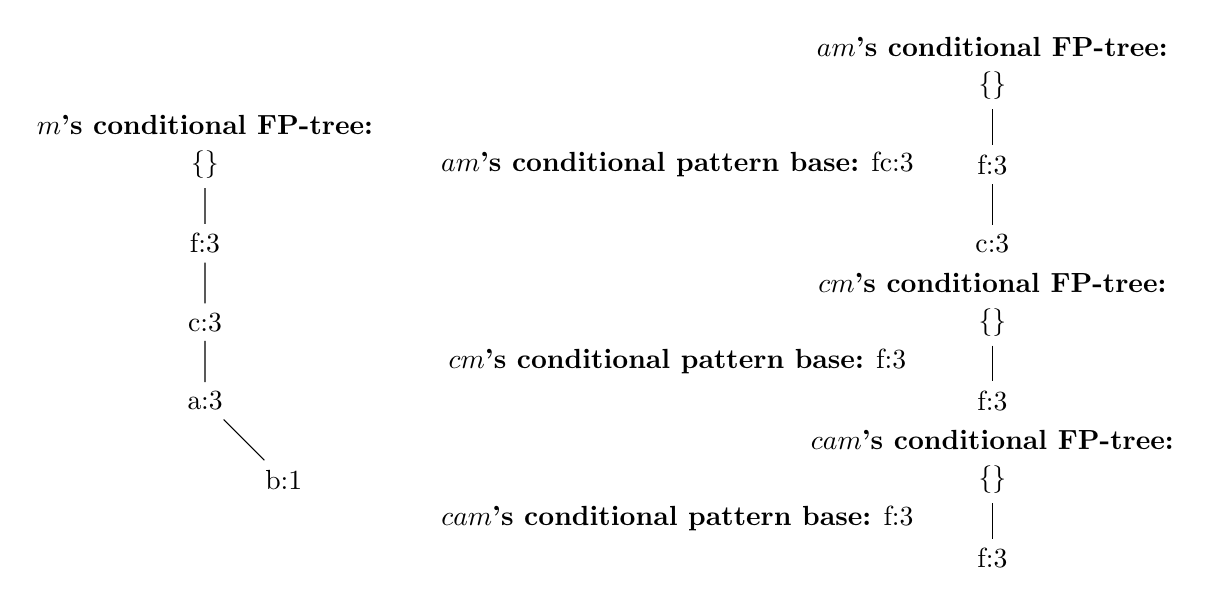
\begin{tikzpicture}
			\node at (0,0.5) (0) {\textbf{$m$'s conditional FP-tree:}};
			\node at (0,0) (0) {$\{\}$};
			\node at (0,-1) (f3) {f:3};
			\node at (0,-2) (c3) {c:3};
			\node at (0,-3) (a3) {a:3};
			\node at (1,-4) (b1) {b:1};
			\draw (0)--(f3)--(c3)--(a3)--(b1);

			\node at (6,-0) (r0) {$am$\textbf{'s conditional pattern base:} fc:3};
			\node at (6,-2.5) (r0) {$cm$\textbf{'s conditional pattern base:} f:3};
			\node at (6,-4.5) (r0) {$cam$\textbf{'s conditional pattern base:} f:3};

			\node at (10,1.5) (0) {\textbf{$am$'s conditional FP-tree:}};
			\node at (10,1) (r0) {$\{\}$};
			\node at (10,0) (rf3) {f:3};
			\node at (10,-1) (rc3) {c:3};
			\draw (r0)--(rf3)--(rc3);

			\node at (10,-1.5) (0) {\textbf{$cm$'s conditional FP-tree:}};
			\node at (10,-2) (rr0) {$\{\}$};
			\node at (10,-3) (rrf3) {f:3};
			\draw (rr0)--(rrf3);

			\node at (10,-3.5) (0) {\textbf{$cam$'s conditional FP-tree:}};
			\node at (10,-4) (rrr0) {$\{\}$};
			\node at (10,-5) (rrrf3) {f:3};
			\draw (rrr0)--(rrrf3);
		\end{tikzpicture}
	}
\end{frame}

\begin{frame}{A Special Case: Single Prefix Path in FP-tree (I)}
	\centering
	\begin{itemize}
		\item \textbf{Suppose a (conditional) FP-tree $T$ has a shared single
			      prefix-path $P$.}
		\item Mining can be decomposed into two parts.
		      \begin{itemize}
			      \item Reduction of the single prefix path into one node.
			      \item Concatenation of the mining results of the two parts.
		      \end{itemize}
	\end{itemize}
	\centering
	\scalebox{0.9}{
		\begin{tikzpicture}
			\node at (0,0) (0) {$\{\}$};
			\node at (0,-0.7) (a1n1) {$a_1:n_1$};
			\node at (0,-1.4) (a2n2) {$a_2:n_2$};
			\node at (0,-2.1) (a3n3) {$a_3:n_3$};
			\node at (-0.7,-2.8) (b1m1) {$b_1:m_1$};
			\node at (0.7,-2.8) (c1k1) {$c_1:k_1$};
			\node at (0,-3.5) (c2k2) {$c_2:k_2$};
			\node at (1.4,-3.5) (c3k3) {$c_3:k_3$};
			\draw (0)--(a1n1)--(a2n2)--(a3n3)--(b1m1);
			\draw (a3n3)--(c1k1);
			\draw (c1k1)--(c2k2);
			\draw (c1k1)--(c3k3);
			\node at (2.1,-2.1) (join) {$\rightarrow$};
			\node at (3.5,-2.1) (r1) {$r_1$};
			\node at (4,-2.1) (r1) {$=$};
			\node at (5,0) (20) {$\{\}$};
			\node at (5,-0.7) (2a1n1) {$a_1:n_1$};
			\node at (5,-1.4) (2a2n2) {$a_2:n_2$};
			\node at (5,-2.1) (2a3n3) {$a_3:n_3$};
			\draw (20)--(2a1n1)--(2a2n2)--(2a3n3);
			\node at (7,-2.1) (r1) {$\oplus$};
			\node at (8.4,-2.1) (30) {$r_1$};
			\node at (8.1,-2.8) (b1m1) {$b_1:m_1$};
			\node at (9.5,-2.8) (c1k1) {$c_1:k_1$};
			\node at (8.4,-3.5) (c2k2) {$c_2:k_2$};
			\node at (9.9,-3.5) (c3k3) {$c_3:k_3$};
			\draw (30)--(c1k1)--(c3k3);
			\draw (30)--(b1m1);
			\draw (c1k1)--(c2k2);
		\end{tikzpicture}
	}
\end{frame}

\begin{frame}{A Special Case: Single Prefix Path in FP-tree (II)}
	\centering
	\begin{itemize}
		\item \textbf{Completeness.}
		      \begin{itemize}
			      \item Preserve complete information for frequent-pattern mining.
			      \item Never break a long pattern of any transaction.
		      \end{itemize}
		\item \textbf{Compactness.}
		      \begin{itemize}
			      \item Reduce irrelevant info - infrequent items are removed.
			      \item Items in frequency-descending order.
			            \begin{itemize}
				            \item The more frequently occurring, the more likely to be
				                  shared.
			            \end{itemize}
			      \item Never larger than the original database.
			            \begin{itemize}
				            \item Not counting node links and the count fields.
			            \end{itemize}
		      \end{itemize}
	\end{itemize}
\end{frame}

\begin{frame}{The FP-growth Mining Method}
	\centering
	\begin{itemize}
		\item \textbf{Idea: FP-growth.}
		      \begin{itemize}
			      \item Recursively grow frequent patterns by pattern and database
			            partition.
		      \end{itemize}
		\item \textbf{Method:}
		      \begin{itemize}
			      \item For each frequent item, construct its conditional pattern
			            base, \\
			            and then its conditional FP-tree.
			      \item Repeat the process on each newly created conditional FP-tree.
			      \item Until the resulting FP-tree is empty, or it contains only one
			            path.
			            \begin{itemize}
				            \item Single path will generate all the combinations of its
				                  sub-paths, \\
				                  each of which is a frequent pattern.
			            \end{itemize}
		      \end{itemize}
	\end{itemize}
\end{frame}

\begin{frame}{Scaling FP-growth by Database Projection}
	\centering
	\begin{itemize}
		\item \textbf{What if FP-tree does not fit in memory?}
		      \begin{itemize}
			      \item DB projection.
		      \end{itemize}
		\item \textbf{First partition database into a set of projected DBs.}
		\item \textbf{Then construct and mine FP-tree for each projected DB.}
		\item \textbf{Parallel-projection vs. partition-projection techniques:}
		      \begin{itemize}
			      \item \textbf{\color{airforceblue}Parallel projection:}
			            \begin{itemize}
				            \item Project the DB in parallel for each frequent item.
				            \item Parallel projection is space costly.
				            \item All the partitions can be processed in parallel.
			            \end{itemize}
			      \item \textbf{\color{airforceblue}Partition projection:}
			            \begin{itemize}
				            \item Partition the DB based on the ordered frequent items.
				            \item Passing the unprocessed parts to the subsequent
				                  partitions.
			            \end{itemize}
		      \end{itemize}
	\end{itemize}
\end{frame}

\begin{frame}{Partition-based Projection}
	\centering
	\scalebox{0.9}{
		\begin{tikzpicture}
			\node at (-4.05,0) {\textbf{Parallel proj. needs much disk space.}};
			\node at (-4.75,-0.5) {\textbf{Partition projection saves it.}};
			\node at (0,-0) (0) {
				\begin{tabular}{|c|}
					\hline
					\textbf{Tran. Db} \\\hline
					fcamp             \\
					fcabm             \\
					fb                \\
					cbp               \\
					fcamp             \\\hline
				\end{tabular}
			};
			\node at (-6,-2.5) (1) {
				\begin{tabular}{|c|}
					\hline
					\textbf{p-proj. DB} \\\hline
					fcam                \\
					cb                  \\
					fcam                \\\hline
				\end{tabular}
			};
			\node at (-3.5,-2.5) (2) {
				\begin{tabular}{|c|}
					\hline
					\textbf{m-proj. DB} \\\hline
					fcab                \\
					fca                 \\
					fca                 \\\hline
				\end{tabular}
			};
			\node at (-1,-2.5) (3) {
				\begin{tabular}{|c|}
					\hline
					\textbf{b-proj. DB} \\\hline
					f                   \\
					cb                  \\
					$\ldots$            \\\hline
				\end{tabular}
			};
			\node at (1.5,-2.5) (4) {
				\begin{tabular}{|c|}
					\hline
					\textbf{a-proj. DB} \\\hline
					fc                  \\
					$\ldots$            \\\hline
				\end{tabular}
			};
			\node at (4,-2.5) (5) {
				\begin{tabular}{|c|}
					\hline
					\textbf{c-proj. DB} \\\hline
					f                   \\
					$\ldots$            \\\hline
				\end{tabular}
			};
			\node at (6.5,-2.5) (6) {
				\begin{tabular}{|c|}
					\hline
					\textbf{f-proj. DB} \\\hline
					$\ldots$            \\\hline
				\end{tabular}
			};
			\node at (-3.5,-4.5) (10) {
				\begin{tabular}{|c|}
					\hline
					\textbf{am-proj. DB} \\\hline
					fc                   \\
					fc                   \\
					fc                   \\\hline
				\end{tabular}
			};
			\node at (-1,-4.5) (11) {
				\begin{tabular}{|c|}
					\hline
					\textbf{cm-proj. DB} \\\hline
					f                    \\
					f                    \\
					f                    \\\hline
				\end{tabular}
			};
			\draw[->] (0)--(1);
			\draw[->] (0)--(2);
			\draw[->] (0)--(3);
			\draw[->] (0)--(4);
			\draw[->] (0)--(5);
			\draw[->] (0)--(6);
			\draw[->] (2)--(10);
			\draw[->] (2)--(11);
			\draw[->, color=airforceblue] (-5.5,-2.3) -- (-3.8,-2.7);
			\draw[->, color=airforceblue] (-5.5,-3.1) -- (-3.8,-3.1);
			\draw[->, color=airforceblue] (-5.5,-2.7) to [out=-20,in=-180]
			(-1.2,-2.7);
			\draw[->, color=airforceblue] (-3.1,-2.3) to [out=20,in=-210]
			(-3.8,-4.3);
			\draw[->, color=airforceblue] (-3.1,-2.7) to [out=20,in=-210]
			(-3.8,-4.7);
			\draw[->, color=airforceblue] (-3.1,-2.7) to [out=20,in=-210]
			(1.2,-2.5);
			\draw[->, color=airforceblue] (1.7,-2.5) -- (3.7,-2.5);
			\draw[->, color=airforceblue] (-3.1,-3.2) to [out=20,in=-210]
			(-3.8,-5.2);
			\draw[->, color=airforceblue] (-3.3,-5.15) -- (-1.2,-5.15);
			\draw[->, color=airforceblue] (-3.3,-4.7) -- (-1.2,-4.7);
			\draw[->, color=airforceblue] (-3.3,-4.25) -- (-1.2,-4.25);
		\end{tikzpicture}
	}
\end{frame}

\begin{frame}{Advantages of the FP-growth Approach}
	\begin{itemize}
		\item \textbf{Divide-and-conquer:}
		      \begin{itemize}
			      \item Decompose both the mining task and DB according
			            to the frequent patterns obtained so far.
			      \item This leads to focused search of smaller databases.
		      \end{itemize}
		\item \textbf{Other factors:}
		      \begin{itemize}
			      \item No candidate generation, no candidate test.
			      \item Compressed database: FP-tree structure.
			      \item No repeated scan of entire database.
			      \item Basic ops: counting local frequent items and building sub
			            FP-tree,\\
			            no pattern search and matching.
		      \end{itemize}
	\end{itemize}
\end{frame}

\begin{frame}{ECLAT: Mining by Exploring Vertical Data Format}
	\begin{itemize}
		\item \textbf{Vertical format: $t(AB) = \{T_{11},T_{25},\ldots\}$}
		      \begin{itemize}
			      \item Tid-list: list of transaction ids containing an itemset.
		      \end{itemize}
		\item \textbf{Deriving frequent itemsets based on vertical
			      intersections.}
		      \begin{itemize}
			      \item $t(X) = t(Y): \qquad$ \hphantom{.} $X$ and $Y$ always happen
			            together.
			      \item $t(X) \implies t(Y):\quad $ transaction having $X$ always has
			            $Y$.
		      \end{itemize}
		\item \textbf{Using diffset to accelerate mining.}
		      \begin{itemize}
			      \item Only keep track of differences of tids.
			      \item $t(X) = \{T_1,T_2,T_3\}$, $t(XY) = \{T_1,T_3\}$.
			      \item Diffset $(XY,X) = \{T_2\}$.
		      \end{itemize}
		\item \textbf{ECLAT} (Zaki et al., KDD'97)
		\item \textbf{Mining closed itemsets using vertical format: CHARM}
		      (Zaki \& Hsiao, SDM'02)
	\end{itemize}
\end{frame}

\begin{frame}{Mining Closed Itemsets: CLOSET (I)}
	\begin{columns}[c]
		\begin{column}{0.6\textwidth}
			\begin{itemize}
				\item \textbf{F-list: list of all frequent items \\ in
					      support-ascending order.}
				      \begin{itemize}
					      \item F-list: d-a-f-e-c.
				      \end{itemize}
				\item \textbf{Divide search space.}
				      \begin{itemize}
					      \item Itemsets having d.
					      \item Itemsets having d but not a, etc.
				      \end{itemize}
				\item \textbf{Find closed itemsets recursively.}
				      \begin{itemize}
					      \item Every transaction having d also has $cfa \implies
						            cfad$ is a closed itemset.
					      \item (Pei, Han \& Mao, DMKD'00)
				      \end{itemize}
			\end{itemize}
		\end{column}
		\begin{column}{0.25\textwidth}
			\begin{tabular}{|c|c|}
				\hline
				TID & Items     \\\hline
				10  & a,c,d,e,f \\\hline
				20  & a,b,e     \\\hline
				30  & c,e,f     \\\hline
				40  & a,c,d,f   \\\hline
				50  & c,e,f     \\\hline
			\end{tabular}
		\end{column}
	\end{columns}
\end{frame}

\begin{frame}{Mining Closed Itemsets: CLOSET (II)}
	\begin{itemize}
		\item \textbf{Itemset merging:.}
		      \begin{itemize}
			      \item If $Y$ appears in each occurrence of $X$, then $Y$ is merged
			            with $X$.
		      \end{itemize}
		\item \textbf{Sub-itemset pruning:}
		      \begin{itemize}
			      \item If $X \subset Y$ and $\text{sup}(X) = \text{sup}(Y),$ $X$ and
			            all of $X$'s\\
			            descendants in the set enumeration tree can be pruned.
		      \end{itemize}
		\item \textbf{Item skipping:}
		      \begin{itemize}
			      \item If a local frequent item has the same support in several
			            header tables at different levels, \\
			            one can prune it from the header table at higher levels.
		      \end{itemize}
		\item \textbf{Efficient subset checking.}
	\end{itemize}
\end{frame}

\begin{frame}{MaxMiner: Mining Max-itemsets}
	\begin{columns}[c]
		\begin{column}{0.6\textwidth}
			\begin{itemize}
				\item \textbf{1st scan: find frequent items.}
				      \begin{itemize}
					      \item A, B, C, D, E
				      \end{itemize}
				\item \textbf{2nd scan: find support for:}
				      \begin{itemize}
					      \item AB, AC, AD, AE, \textbf{ABCDE}
					      \item BC, BD, BE, \textbf{BCDE}
					      \item CD, CE, \textbf{CDE}, DE
				      \end{itemize}
				\item \textbf{Potential max-itemsets: ABCDE, BCDE, CDE.}
				\item \textbf{Since BCDE is a max-itemset, no need to check
					      BCD, BDE, CDE in later scan.} (Bayardo, SIGMOD'98)
			\end{itemize}
		\end{column}
		\begin{column}{0.3\textwidth}
			\begin{tabular}{|c|c|}
				\hline
				TID & Items     \\\hline
				10  & A,B,C,D,E \\\hline
				20  & B,C,D,E   \\\hline
				30  & A,C,D,F   \\\hline
			\end{tabular}
		\end{column}
	\end{columns}
\end{frame}
